\documentclass[justified, nofonts, notoc, debug]{tufte-book}

\usepackage{amsmath}
\usepackage{amssymb}
\usepackage{cag}
\usepackage{fancyhdr}
\usepackage{float}
\usepackage{geometry}
\usepackage{graphicx}
\usepackage{epstopdf}
\usepackage{listings}
\usepackage{makeidx}
\usepackage{microtype}
\usepackage{nag}
\usepackage{titlepic}
%\usepackage[usenames,dvipsnames,svgnames,table]{xcolor}

%\usepackage{arevmath}
\usepackage{lmodern}
\usepackage{bera}

\usepackage{hyperref}

%\pagestyle{fancy}

%\geometry{a4paper} % May funkify floating listings

%\definecolor{TUBlue}{RGB}{61,152,222}
%\definecolor{SpartanGreen}{RGB}{24,69,59}


\hypersetup{
    colorlinks=true,
    citecolor=Blue,
    linkcolor=Blue,
    urlcolor=Green
}

\lstset{
  language=fortran,
  basicstyle=\ttfamily,
  commentstyle=\itshape\color{Blue},
  keywordstyle=\bfseries\color{DarkRed},
  stringstyle=\color{Magenta},
  columns=fixed,
  numbers=left,
  numberstyle=\footnotesize\color{lightgray},
  numberblanklines=true,
  showstringspaces=false,
  caption=\lstname,
  firstnumber=auto,
  frame=single,
  rulesepcolor=\color{black},
  gobble=2 % Allow indentation in LaTeX source for readibility
}

\lstdefinestyle{prompt}{
  language=bash,
  caption=,
  commentstyle=\itshape\color{gray},
  keywordstyle=\ttfamily,
  numbers=none,
  frame=none
}

\newcommand{\keyword}[1]{\texttt{\bfseries\color{DarkRed}#1}}
\newcommand{\str}[1]{\texttt{\color{Magenta}#1}}
\newcommand{\Chapter}[2]{\chapter[#1]{#1\\[1ex]\Large#2}} 

\renewenvironment{quote}{\list{}{\leftmargin=8\parindent}\item\relax}{\endlist}

\makeindex

%\widowpenalty=3000
%\clubpenalty=3000

\title{ICCP Coding Manual}
\author{Connor Glosser, Jos Seldenthuis, Chris Verzijl, \\ 
  Erin McGarrity, and Jos Thijssen}
  \titlepic{
    \begin{figure}[b]
      \centering
      \includegraphics[width=0.33\pdfpagewidth]{figures/MSU_logo.pdf} \hfill
      \includegraphics[width=0.33\pdfpagewidth]{figures/TU_logo.pdf}
    \end{figure}
  }

\begin{document}


%\frontmatter
\maketitle

%\newpage
%\null
%\vfill
%\begin{center}
  %\includegraphics[width=0.15\textwidth]{figures/by-nc-sa.eps}
%\end{center}
%This work, including its figures and \LaTeX\ source code, is licensed under the Creative Commons Attribution-NonCommercial-ShareAlike 4.0 International License. 
%To view a copy of this license, visit \url{http://creativecommons.org/licenses/by-nc-sa/4.0/deed.en_US}.

\tableofcontents
%\lstlistoflistings

\include{chapters/Introduction}
\mainmatter
\chapter{Getting your toes wet with Fortran and Linux}
\label{chap:Getting your toes wet}
\begin{quote}\small
  \emph{``1957: John Backus and IBM create FORTRAN. There's nothing funny about IBM or FORTRAN. It is a syntax error to write FORTRAN while not wearing a blue tie.''} \\ \hspace*{\fill}---James Iry
\end{quote}

For this course we recommend using the GNU Fortran compiler, as it is free and of reasonably high quality.\footnote{You're welcome to use the Intel Fortran compiler, which is free on Linux, but remember to change the compiler flags, since they differ from \texttt{gfortran}.} 
Linux is the platform of choice, since it's most suited to programming and high-performance computing.\footnote{As of this writing, 476 of the top 500 supercomputers in the world run some form of Linux.}
OS~X, being a Unix variant, is also an option, but installing the required packages is generally a bit more work.
In these notes we will assume that you're using Ubuntu.\footnote{You can use Ubuntu as a native installation, run it from a flash drive, under a virtual machine, or under Windows using Wubi.
Ask your instructor.}

After booting Ubuntu, you need to install a Fortran compiler.
Open a terminal and at the prompt (the \$) type
\begin{lstlisting}[style=prompt, nolol]
  $ sudo aptitude install gfortran gfortran-doc
\end{lstlisting}
\emph{Note that anything you type in the console is case-sensitive!} 
This command grants \texttt{aptitude} privilieges to search for and then install the \texttt{gfortran} package and its documentation.
You may also find it useful to install the \LaTeX\ typesetting system for writing reports.
You can install it with another call to \texttt{aptitude}:
\begin{lstlisting}[style=prompt, nolol]
  $ sudo aptitude install texlive # or texlive-full for a complete installation
\end{lstlisting}

Once you have \texttt{gfortran} installed, you can start writing programs.
You will generally compile and run your programs from a terminal window (also called a \emph{console}).
A few useful commands are:
\begin{lstlisting}[style=prompt, nolol]
  $ ls              # display the contents of the current directory
  $ ls -l           # display contents with extra details
  $ cp file path    # copy 'file' to 'path'
  $ mv file path    # move 'file' to 'path'
  $ rm file         # remove 'file'
  $ mkdir dir       # create a new directory called 'dir'
  $ cd dir          # change current directory to 'dir'
  $ rmdir dir       # remove directory 'dir' (only if it's empty)
  $ rm -r dir       # remove directory 'dir' (even if it's not empty)
  $ man cmd         # provide documentation on 'cmd'
\end{lstlisting}

For your first program, open a terminal, create a directory for ICCP files and open your first Fortran file by typing
\begin{lstlisting}[style=prompt, nolol]
  $ mkdir iccp          # create a new directory called 'iccp'
  $ cd iccp             # move to the new directory
  $ gedit myprog.f90    # open a text editor with the file 'myprog.f90'
\end{lstlisting}
The gedit text editor pops open in which you can type the program in \autoref{lst:myProg}.
It is probably obvious what this program does. However, a few remarks are in order:
\begin{itemize}
  \item The program starts with a declaration of variables.
    \texttt{\keyword{real}(8)} denotes a floating-point variable with double (8 byte) precision. 
    Similarly, \keyword{integer} denotes an integer number.\footnote{Fortran intrisic types include \keyword{logical}, \keyword{integer}, \keyword{real}, \keyword{complex}, and \keyword{character} data.}
    Not specifying a size generally defaults to 4-byte precision.
    \keyword{implicit none} prevents Fortran from trying to infer the type from the variable name, which is a major source of bugs---\emph{always include this!}
  \item The attribute \keyword{parameter} specifies that we are declaring a constant.
    Although Fortran is case-insensitive, it is considered good practice to always use uppercase names for constant variables.
  \item Note the calculation of $\pi$ as $4\arctan(1)$---convenient and accurate.
  \item Single-precision (4 byte) floating-point numbers can be written as \texttt{0.1} or \texttt{1e-1} (scientific notation). 
    For double-precision numbers, use \texttt{d} instead of \texttt{e} in scientific notation, \eg, \texttt{1d-1}. 
    It is also possible to specify the precision as a suffix: \texttt{1.0\_4} for single and \texttt{1.0\_8} for double precision. 
    This also works for integers.
  \item \texttt{\keyword{integer} :: fibonacci(N)} allocates an array of 20 
    integers, with the array index\footnote{Array indices can start at 
    any integer by specifying a lower and upper bound separated with a colon.} running from 1 to 20.
  \item `\texttt{*}' is multiplication, `\texttt{**}' is exponentiation.
  \item The \keyword{print} statement on line 24 contains the formatting string \str{"(4I6)"}. 
    This tells Fortran to print 4 records of integer type per line, each taking up 6 characters.
    Format strings for other datatypes include E$w.d$ (real -- decimal form), ES$w.d$ (real -- scientific form), EN$w.d$ (real -- engineering form), L$w$ (logical), and A (characters). Here, $w$ gives the width of a record and $d$ gives the number of places right of the decimal.
  \item Comments in Fortran start with `\texttt{!}' and last until the end of the line.
  \item Dividing integers \textcolor{red}{\textbf{results in an integer}}, so \texttt{3 / 2 = 1} instead of 1.5 as you might expect. 
    Multiplying by \texttt{1d0} on line 27 forces Fortran to do a double-precision floating-point calculation.
\end{itemize}
Now we compile and run the program.
Compiling means translating the Fortran source code into machine code (processor instructions).
This can be done by simply typing
\begin{verbatim}
$ gfortran myprog.f90
\end{verbatim}
which will result in the executable file \texttt{a.out}.
This is the default name for the output.
You can specify a different name by compiling with
\begin{verbatim}
$ gfortran myprog.f90 -o myprog
\end{verbatim}
which results in a program with the name \texttt{myprog}.
During compilation, the compiler may generate error messages and warnings.
The errors must be fixed before an actual running program is produced, and it is good practice to also make sure no warnings are generated.

The compilation process can be tuned by passing certain command-line arguments to the compiler.
We recommend using always at least the following:
\begin{verbatim}
$ gfortran -Wall -Wextra -march=native -O3 myprog.f90 -o myprog
\end{verbatim}
\begin{itemize}
  \item \texttt{-Wall} and \texttt{-Wextra} turn on all warnings.
    This may generate a lot of messages, but fixing them all leads to much cleaner code.
    This can be a huge time saver; not only for you, but also for your instructors!
    If your program doesn't behave as expected, first try to fix all warnings before asking your instructors for help.
  \item \texttt{-march=native} tells the compiler to generate machine code using all available processor instructions on your machine.
    On moderns CPUs this leads to much faster code, since \texttt{gfortran} can use vector instructions.
    The downside is that it can result in executables that will not run on a different machine.
  \item \texttt{-O3} turns on all optimizations.
    This increases the compilation time significantly, although it should still be fast enough for the programs you'll write in ICCP.
    The runtime of your program, on the other hand, will dramatically decrease.
    The only reason not to use this flag is that it might interfere with the debugger (see below).
  \item A possible additional optimization flag is \texttt{-ffast-math}.
    This flag enables floating-point optimizations which might reduce accuracy or result in incorrect behavior, especially in situations such as divide-by-zero.
    We therefore recommend not using this flag until you have verified that your program produces the correct results.
    After that you can use it to make your program faster, but do check that it still behaves correctly.
  \item Finally, if your code starts throwing segmentation faults (segfaults), consider using the \texttt{-fbounds-check} flag.
    Segfaults usually occur because you've run an index off the end of an array, so compiling with this flag turns on runtime bounds checking (at the expense of significantly reduced performance).
\end{itemize}
If the program compiled correctly, you can run it by typing \texttt{./a.out} or \texttt{./myprog}.
Note that \texttt{./} specifies the \emph{path}, \ie, the location where to find the program.
The dot means the current directory, and the slash separates directories and file names (like the backslash in DOS and Windows).

\lstinputlisting[float=h!,label=lst:myProg]{examples/myProg.f90}

\include{chapters/Structuring_your_code}
\chapter{The magic of Makefiles}
\label{chap:Makefiles}

Once your programs become larger, it is convenient to split the source code into several files.
However, to obtain a running program, each of these files has to be compiled separately (resulting in a \emph{relocatable object file}, with extension \texttt{.o}) and then combined (linked) into a single program.
Doing this by hand quickly becomes tedious, so we resort to using Makefiles.
We create a file called \texttt{Makefile} that contains all compiler invocations, and then we can compile the program by simply typing
\begin{verbatim}
$ make
\end{verbatim}
Similarly, we can remove all compiler-generated files with
\begin{verbatim}
$ make clean
\end{verbatim}
The \texttt{make} program is smart enough to only compile files that have changed; so if you just fixed a bug in \texttt{file6.f90}, it will only recompile that file (generating \texttt{file6.o}) and perform the linking step, without touching the other files.

\lstinputlisting[language=,showtabs=true,float=htb,label=lst:example_makefile]{examples/example_makefile}
So, what does a \texttt{Makefile} look like? As an example, let's go through \autoref{lst:example_makefile} step by step.
\begin{itemize}
  \item The first lines declare a few variables for later use.
    \texttt{FC} is set to the Fortran compiler \texttt{gfortran}, \texttt{FFLAGS} contains the compiler flags and \texttt{LDFLAGS} the linker flags.
    The \texttt{COMPILE} and \texttt{LINK} variables combine these to get the compile and link commands.
  \item Most non-trivial programs make use of several function libraries, such as the Linear Algebra PACKage (LAPACK).
    These libraries are stored under \texttt{/usr/lib} and have filenames such as \texttt{liblapack.a} or \texttt{liblapack.so}.
    You can link such a library with your program by specifying the \texttt{-llapack} argument to the linker.
    Note that you have to omit both \texttt{lib} and the extension (\texttt{.a} or \texttt{.so}) from the library name.
    Since libraries have to appear after the object files for the linker, they are specified in the separate variable \texttt{LIBS}.
    If the library cannot be found in the system paths, you can tell the compiler to search for it in the directory \texttt{\emph{PATH}} by adding the option \texttt{-L\emph{PATH}} to \texttt{LDFLAGS}, \eg, \texttt{LDFLAGS = -L\$HOME/mylib}.
  \item Makefiles are built around rules, which have the form `\texttt{\emph{target}: \emph{dependencies}}' followed by some lines with the commands needed to create the target from the dependencies.
    Except for a few special targets, such as \texttt{all} and \texttt{clean}, \texttt{make} will assume the target is a file, and try to recreate it if the target is older than the dependencies.
    \emph{Note that the lines with the build commands must start with a tab character, not spaces!}
  \item If \texttt{make} is invoked without any parameters, the default target is the first entry in the \texttt{Makefile} (in this case \texttt{all}), which depends on \texttt{myprog} here.
    \texttt{myprog} in turn depends on the list of object files in \texttt{\$(OBJS}).
    This is the reason we only specified the object files and not the source code files.
    The executable is generated by invoking the linker, which combines the object files with the external libraries.
    In the \texttt{Makefile}, \texttt{\$@} is an alias for the target.
    On line 17, for example, \texttt{\$@} is replaced by \texttt{myprog} when running \texttt{make}.
    Similarly, \texttt{\$\^} is an alias for all dependencies, in this case the list \texttt{\$(OBJS)}.
  \item Since we don't want to specify a separate rule for every object file, we use \emph{wildcards}.
    \texttt{\%.o: \%.f90} means every object file ending in \texttt{.o} depends on the corresponding source file, ending in \texttt{.f90}.
    \texttt{\$<} on the command line is an alias for the first prerequisite, in this case the source file.
    The \texttt{-c} option tell the compiler to only perform the compilation step to create an object file, and to skip linking.
    Note that the object files are compiled in the order specified in \texttt{\$(OBJS)}.
    This means that if the program file \texttt{myprog} depends on the module \texttt{mymod}, \texttt{mymod.o} needs to be listed before \texttt{myprog.o}.
  \item The special target \texttt{clean} is used to delete all compiler-generated files.
    This includes the executable \texttt{myprog}, the object files listed in \texttt{\$(OBJS)} and any automatically generated module files (with extension \texttt{.mod}).
\end{itemize}
In the rest of these notes we will assume that you have created a \texttt{Makefile} for each project based on this template.

\Chapter{Debugging}{(or, where you'll spend 90\% of your time)}
\label{chap:Debugging}

\begin{quote}\small
  \emph{``Everyone knows that debugging is twice as hard as writing a program in the first place.
  So if you're as clever as you can be when you write it, how will you ever debug it?'' \\ \\
  ``The most effective debugging tool is still careful thought, coupled with judiciously placed print statements.''} \\\hspace*{\fill}---Brian Kernighan
\end{quote}
The \texttt{MyProg} program does not contain any bugs (fingers crossed) and works as expected.
However, any non-trivial program will be buggy after your first attempt at writing it.
\emph{In this course you will spend the majority of your time debugging your algorithms and your code, not on the actual writing!} To ease your pain, we recommend following the golden rules of debugging:
\begin{itemize}
  \item\textbf{Always fix the first error first.} Errors have a tendency to cascade, with a simple typo early on generating loads of errors in the rest of your program.
    If you find yourself with a ton of unmanageable issues, use the \texttt{-Wfatal-errors} flag to halt compilation after the first error so you can fix them individually.
  \item\textbf{Don't ignore warnings.} Warnings are often an indication that your code doesn't actually do what you think it does.
    And if it does happen to work, it's an indication of bad programming practice, or worse, style.
    You can use the \texttt{-Werror} flag to elevate warnings into errors, forcing you to fix them before the compiler will produce an executable.
  \item\textbf{Test early, test often.} No matter how large the project, always start with a trivial program and make sure that works.
    Then add functionality bit by bit, each time making sure it compiles and works.
  \item\textbf{Produce lots of output.} You might think that there can't possibly be a bug in that beautiful expression, but you're wrong.
    There are countless innocuous subtleties to programming that can result in inaccuracies or unintended side effects.
    Test your program by printing the intermediate results.
  \item\textbf{Keep a rubber ducky on your desk.} You've been staring at your code for hours, it's obviously correct, yet it doesn't work.
    In that case the best thing to do is to try and explain your code to someone else.
    It doesn't matter who it is; they don't have to understand Fortran, or even programming in general.
    It can be your partner, your mother, your dog, or even a rubber ducky.
    Just explain it line-by-line; ten to one says you'll find the bug.
\end{itemize}
Even if you do follow these rules---\emph{and you should!}---you will run into bugs that you don't understand.
Often they can be fixed by backtracking and checking every intermediate step, but bugs can be elusive.
In those cases a debugger comes in handy.
To use a debugger under Ubuntu, install the \texttt{gdb} and \texttt{ddd} packages.
You'll also need to compile your program with the \texttt{-g} flag to generate debug symbols, and turn off any optimizations as they might reorder expressions in your code, \eg,
\begin{verbatim}
$ gfortran -Wall -Wextra -march=native -g myprog.f90 -o myprog
\end{verbatim}
If the program compiles, you can invoke the debugger with
\begin{verbatim}
$ ddd ./myprog
\end{verbatim}
This will open a window showing the source code of your program and a GDB console (the actual debugger).
You can run the program by pressing the `Run' button, and interrupt a running program with `Interrupt'.
You can also insert so-called breakpoints into your program by right-clicking on a line and selecting `Set Breakpoint'.
If you then run your program, it will execute until it encounters the breakpoint, where it will pause.
You can then step through your code by clicking `Step' or `Next'.
`Step' will move to the next statement in your code.
`Next' does the same, but it will step over subroutines instead of entering them.
You can inspect variables by right-clicking on the name and selecting `Print x' or `Display x'.

Play around with the debugger for a while until you're comfortable using it.
It will come in very handy when you're hunting bugs, and as we said before, that's what you'll be spending most of your time on.

\Chapter{Optimization}{(or, where you \emph{shouldn't} spend 90\% of your time)}
%\chapter[Optimization]{Optimization (or where you \emph{shouldn't} spend 90\% of your time)}
\label{chap:Optimization}

\begin{quote}\small
\emph{``Premature optimization is the root of all evil.''} \\ \hspace*{\fill}---Donald E.\ Knuth
\end{quote}
\begin{quote}\small
\emph{``Rules of Optimization: \\ Rule 1: Don't do it. \\ Rule 2 (for experts only): Don't do it yet.''} \\ \hspace*{\fill}---Michael A.\ Jackson
\end{quote}
Impatience is the most important characteristic of a good programmer.
However, this does result in a tendency to focus too much or too early on optimizing code. Don't.
Always make sure your code is correct and readable before you try to make it faster.
And if you do, the golden rule is: \emph{don't optimize your code, optimize your algorithms.}
This may seen counter-intuitive; after all, what's wrong with fast code?
However, modern CPUs are complex beasts, and unless you're an expert, it's not at all obvious which expressions result in the fastest code.
This also means that a lot of tricks that used to be valid ten years ago no longer are.
Let's look at a few examples:
\begin{itemize}
  \item\textbf{Division is slower than multiplication by an inverse.} Although true, optimizing for this results in code that is hard to read, and possibly less accurate.
    Besides, when you're using the \texttt{-ffast-math} option, \texttt{gfortran} will do this for you.
    A similar observation holds for exponentiation; it is slower than multiplication in general, but \texttt{gfortran} will automatically convert \texttt{x**2} to \texttt{x * x}, provided the exponent is \keyword{integer}.
  \item\textbf{Unwinding small loops reduces overhead.} Common wisdom says that
\begin{lstlisting}[caption=, nolol]
  do i = 1, 3
      call do_something(i)
  end do
\end{lstlisting}
    is slower than
\begin{lstlisting}[caption=, nolol]
  call do_something(1)
  call do_something(2)
  call do_something(3)
\end{lstlisting}
    because of the overhead of the loop.
    Although again true in principle, modern CPUs use branch prediction, which reduces the overhead.
    Moreover, unwinding loops results in more machine code, which might actually hurt performance if it no longer fits in the CPU instruction cache.
    When you compile with \texttt{-march=native}, the compiler knows about the CPU limitations and will decide whether loop unwinding is the smart thing to do.
  \item\textbf{Calculate everything only once.} Let's say that $x^2$ occurs four times in your expression, then it makes sense to calculate \texttt{x2 = x**2} separately and use the result four times, right? Possibly yes, but only if it improves readability.
    Common subexpression elimination is something compilers have done for ages, so again \texttt{gfortran} will do this for you.
\end{itemize}
There are countless more examples, but I think you get the idea.
In short: optimize for readability; write clean code and let the compiler worry about the rest.
Unless you're intimately familiar with things like cache misses, branch prediction and vector instructions, you won't be able to outsmart the compiler.

\section{Some optimizations you are allowed to use}

That being said, there are a few general rules that will prevent your code from accidentally becoming horrendously slow:
\begin{itemize}
  \item\textbf{Don't reinvent the wheel.} Don't try to write your own matrix multiplication routine, use \texttt{matmul}, or the routines from BLAS (see the \nameref{chap:Linear algebra} appendix).
    Fortran has many built-in numerical functions that are much faster than anything you'll be able to write---use them! (Google `Fortran intrinsics' to get an overview.)
  \item\textbf{Use array operations.} You can add two arrays by writing
\begin{lstlisting}[caption=, nolol]
  do i = 1, n
      do j = 1, m
          c(i, j) = a(i, j) + b(i, j)
      end do
  end do
\end{lstlisting}
or simply by writing \texttt{c = a + b}.
Guess which is both faster and more readable?
  \item\textbf{Keep inner loops small.} The code inside loops, especially in nested loops, is executed many times.
    This code will likely be the bottleneck of your program, so it makes sense to concentrate your optimization efforts there.
    Move as much code out of the inner loop as possible.
  \item\textbf{Don't use system calls in nested loops.} Certain operations, such as allocating memory, or writing to the screen or disk, require a system call---a function call to the underlying operating system.
    Such calls are expensive, so try to avoid them in nested loops.
    Especially disk I/O is slow.
    Luckily, modern operating systems are smart enough to buffer these operations, but they can still become a bottleneck.
  \item\textbf{Be smart about memory usage.} First, don't use more memory than you need, especially more memory than is physically available.
    That will result in paging (storing and retrieving data from disk), which is orders of magnitude slower than direct memory access.
    Second, think about memory layout.
    Fortran uses column-major ordering for arrays.\footnote{MATLAB and R adopt the same convention as Fortran; C, Python, and Mathematica use row-major ordering.}
    This means that the array
    \begin{equation*}
    \begin{bmatrix}
        a & b & c & d \\
        e & f & g & h \\
        i & j & k & l
    \end{bmatrix}
    \end{equation*}
    is actually stored in memory as $\left[a,e,i,b,f,j,c,g,k,d,h,l\right]$.
    Because of this, operations within a single column are much faster than operations within a single row; the processor can easily load a whole column into the cache, but not a whole row.
    It is therefore important to carefully consider your array layout.
    For example, if you have an array containing the coordinates of many particles, then a $3\times n$ layout will be more efficient than $n\times 3$.
    In the former, the $x$, $y$ and $z$ coordinates are close together in memory, meaning that operations on single particles will be fast.
\end{itemize}
These optimizations are more about preventing your code from becoming unnecessarily slow, than trying to squeeze the last drop of performance out of it.
Besides, low-level optimizations generally yield only about a factor of 2 speedup, and that's if you know what you're doing.
To see real speedups, you're better off profiling your code to determine bottlenecks and optimizing your algorithms by improving scalability.

\section{Scalability; or, the importance of big O}

If you want your program to be fast, choose your algorithms carefully.
The fact that you can approximate an integral by a simple sum does not mean that's the best way to do it.
In fact, the \naive\ approach is often the worst method, both in terms of computational complexity, \ie, how much more expensive the calculation becomes when you increase the size of the problem, and numerical accuracy, \ie, how small the error becomes when you increase the number of steps/iterations.
Both the complexity and the accuracy of an algorithm are generally quantified using \emph{big O} notation.
Big O notation is essentially a Taylor expansion of your algorithm; usually in the step size $h$ to approximate the error, or the dimension $n$ to approximate the computation time.
In general, only the highest or lowest power matters, since that will be the dominant term for large $n$ or small $h$.
Different algorithms for solving the same problem are compared by looking at their big O characteristics.
However, scaling is not everything.
Some algorithms, such as the famous Coppersmith-Winograd algorithm for matrix multiplication, scale very well, but have such a large prefactor in their computational cost, that they're inefficient for all but the largest problems.

Long story short; spend some time doing research before you start coding.
Look at different algorithms, compare their accuracies and complexities---don't forget the complexity of implementation!---and only then start writing.
Don't just go for the seemingly obvious approach.
For example, \naively\ integrating an ordinary differential equation (ODE), \eg, using the Euler method, will make an error of order $\mathcal{O}\left(h^2\right)$ at each integration step, giving a total error of $\mathcal{O}(h)$.
Moreover, this method is unstable, meaning that for stiff equations the solution will oscillate wildly and the error grow very large.
The Runge-Kutta method, on the other hand, makes an error of $\mathcal{O}\left(h^5\right)$ per step, giving a total error of $\mathcal{O}\left(h^4\right)$ (which is why it's generally referred to as `RK4').
Additionally, the method is numerically stable.
%Alternatively, the velocity Verlet algorithm has a global error of $\mathcal{O}\left(h^2\right)$, but it is symplectic, \ie, it is time-reversible and conserves (a discrete version of the) energy.
%This makes it ideal for, \eg, molecular dynamics simulations.
Many such methods are significantly more accurate than the Euler method, without being harder to implement.
Furthermore, better scaling of the error means that they need fewer iterations, making them also much faster; it's a win-win.

Numerical analysis is a large field, and it can be quite daunting trying to understand the merits of different methods, or even finding them.
For this, we recommend the book \emph{Numerical Recipes}.
It covers a wide range of topics, focuses on best practices, and does not ignore coding effort when comparing algorithms.
It even includes the full source code of the implementations! We recommend always using it as your starting point, with one exception: linear algebra (see \autoref{chap:Linear algebra}).

We conclude this section with an overview of the computational complexity of certain common operations.
This will give you an idea of the most likely bottleneck in your code.
\begin{itemize}
  \item All scalar operations are $\mathcal{O}(1)$, \ie, constant time.
    Integer operations are much faster than floating-point operations.
    Addition and subtraction are the fastest, followed by multiplication and finally division.
    Functions like \keyword{sqrt}, \keyword{exp}, \keyword{log}, \keyword{sin}, \keyword{cos}, \emph{etc.}, are not always available as single processor instructions, especially for complex numbers, in which case they are implemented as actual function calls.
    It goes without saying that this is much slower than basic arithmetic.
  \item Scaling a vector or a matrix means performing an operation on each element.
    The complexity is therefore $\mathcal{O}(n)$ for vectors and $\mathcal{O}\left(n^2\right)$ for matrices, where $n$ is the dimension.
  \item Vector addition and taking an inner product are $\mathcal{O}(n)$, matrix addition is $\mathcal{O}\left(n^2\right)$.
  \item Matrix-vector multiplication means taking an inner product for each row, so the complexity is $\mathcal{O}\left(n^2\right)$.
  \item Solving a system of linear equations is also $\mathcal{O}\left(n^2\right)$, but the prefactor is much larger than for matrix-vector multiplication.
  \item \Naive\ matrix-matrix multiplication is $\mathcal{O}\left(n^3\right)$.
    Libraries such as BLAS and LAPACK are smarter and do it in $\mathcal{O}\left(n^{\log_2(7)}\right)\approx\mathcal{O}\left(n^{2.807}\right)$.
    Another reason to not write this yourself.\footnote{The Fortran intrinsic \texttt{matmul} is actually implemented using BLAS.}
  \item Taking the inverse of\ a matrix and calculating the eigenvalues/eigenvectors are both $\mathcal{O}\left(n^3\right)$.
    However, eigendecomposition has a much larger prefactor and is therefore significantly slower.
    It is logically the most expensive matrix operation, since all operations on a diagonal matrix are $\mathcal{O}(n)$.
  \item Iterative algorithms like conjugate-gradient or Krylov-subspace methods are supra-\linebreak convergent in the number of iterations, \ie, the error decreases by a constant factor at each iteration.
    They are especially suitable for sparse matrices, since each iteration is $\mathcal{O}(n)$, where $n$ is the number of non-zero elements instead of the dimension.
\end{itemize}



\include{chapters/Debugging}
\include{chapters/Optimization}
\include{chapters/Coding_style}
\include{chapters/Random_numbers}
\appendix
\include{chapters/Linear_algebra}
\include{chapters/Plotting_with_plplot}
\Chapter{Parallel computing}{Employing a thousand monkeys}
\label{chap:Parallel computing}

\begin{quote}\small
  \emph{``Here be dragons.''}
\end{quote}

If you have a multicore processor, or even multiple processors or machines available, one obvious way to speed up your code is to employ multiprocessing.
However, this is a difficult and dangerous endeavor, especially if you don't have any prior experience.
Parallel programs are far more difficult to write and debug than sequential ones, mostly because concurrency introduces entire classes of potential bugs, like race conditions and deadlocks.
Also, even if it does work, it's not always beneficial.
Some algorithms simply don't scale to multiple processors.
\begin{marginfigure}
  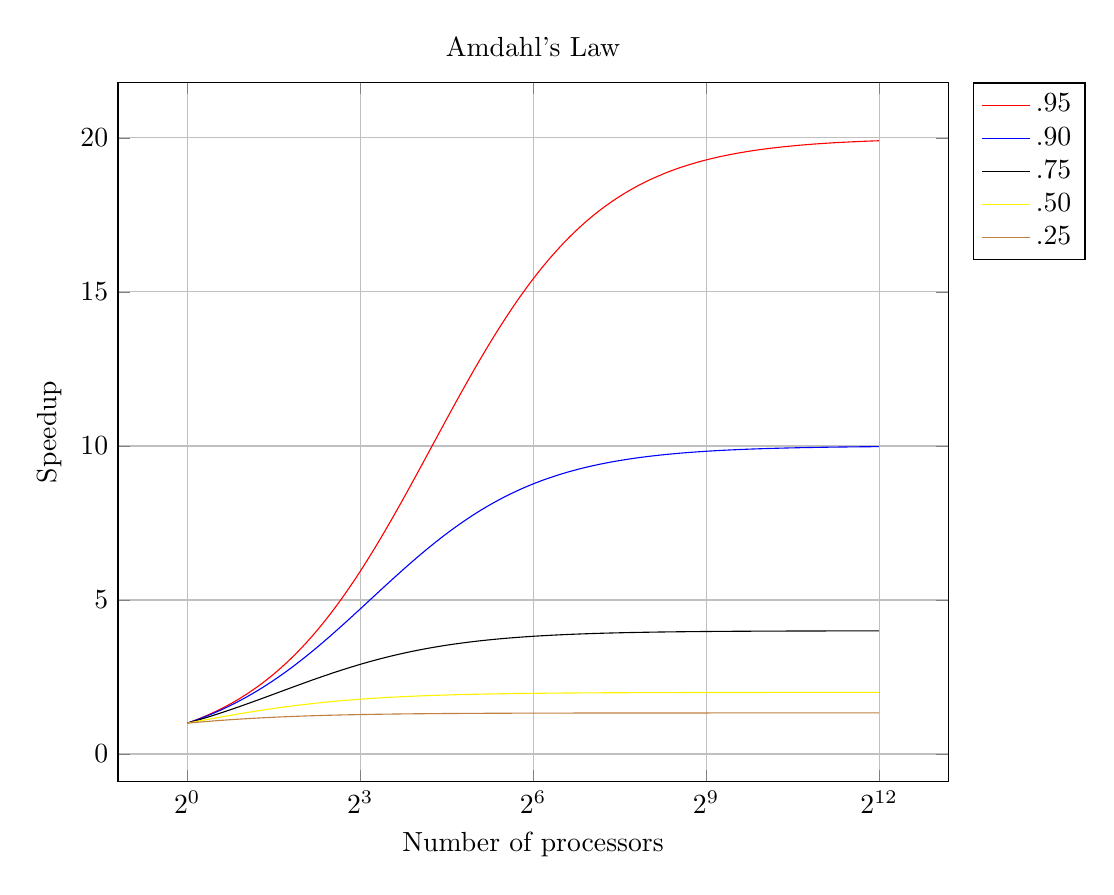
\begin{tikzpicture}
    \begin{axis}[
      title=Amdahl's Law,
      width=\textwidth,
      grid=major,
      xlabel=Number of processors,
      xmode=log,
      log basis x={2},
      xtick={1,8,64,512,4096},
      ylabel=Speedup,
      ylabel near ticks,
      ytick={0,5,10,15,20},
      legend pos=outer north east,
      cycle list name=color list
    ]
    \foreach \p in {.95, .90, .75, .50, .25} {
      \addplot+[
        no marks,
        domain=1:4096,
        samples=201
      ] {1/((1 - \p) + \p/x)};
      \addlegendentryexpanded{$\p$};
    }
    \end{axis}
  \end{tikzpicture}
  \caption{Amdahl's law details the theoretical speedup of a fixed-size algorithm given the fraction of the algorithm that can execute in parallel $(f_p)$ and the number of processors available for computation.}
\end{marginfigure}
Despite its complexity, parallel programming is unavoidable in high-performance computing.
While a true introduction is outside the scope of these notes, we'll give a few guidelines that might help you from accidentally shooting yourself in the foot:
\begin{itemize}
  \item\textbf{Make sure your program works first.} Although this is true for optimizations in general, it is doubly so for parallel programs.
    Programs are much harder to debug when they run in parallel, so leave parallelization for the final step.
  \item\textbf{Check whether the bottleneck in your program benefits from parallelization.} Not every algorithm scales well.
    It would be a waste of time to spend effort parallelizing your code only to discover that it's now actually slower.
  \item\textbf{Use OpenMP.}\footnote{OpenMP is available for C, \Cplusplus{} and Fortran.
    If you are using \Cplusplus, the \emph{Intel Threading Building Blocks} library is a possible alternative; it has high-level support for certain algorithms and data structures.} For ICCP you won't be using supercomputers or systems with multiple nodes.
    Sophisticated libraries like MPI\footnote{Message Passing Interface: a standardized protocol for communications between nodes in a cluster---used on pretty much every supercomputer in the TOP500.} are overkill and introduce needless complexity.
    OpenMP only works on single machines with shared memory, but it is by far the easiest framework to use.
    All you need to do is add \texttt{-fopenmp} to \texttt{FFLAGS} and \texttt{LDFLAGS} in your \texttt{Makefile} and add a few directives to your code.
    For example
\begin{lstlisting}[caption=, nolol]
  !$omp parallel do
  do i = 1, n
      y(i) = x(i) * i
  end do
  !$omp end parallel do
\end{lstlisting}
    will execute the loop in parallel. Use Google for more information on how to use OpenMP.
  \item\textbf{Don't use more threads than you have physical cores.} This may seem like stating the obvious, but it actually happens rather often.
  Most modern Intel processors implement hyper-threading.
  This doubles the apparent number of cores, which helps with task switching when you're running many different programs at once.
  However, for CPU intensive calculations, like the ones you'll be running, the threads will be competing for the available physical cores.
  In that case doubling the number of threads will actually harm performance.
\end{itemize}


\chapter{Revision control}
\label{chap:Revision control}

\begin{quote}
\emph{``And then there's \texttt{git rebase --interactive}, which is a bit like \texttt{git commit --amend} hopped up on acid and holding a chainsaw---completely insane and quite dangerous but capable of exposing entirely new states of mind."} \\ \hspace*{\fill}---Ryan Tomayko
\end{quote}

A revision control system is perhaps the third most useful tool to a programmer after only the editor and compiler.
The idea is simple: you give a piece of software a description of recent changes you've made to your code, and that software will efficiently log the changes and description for you to view and optionally undo should you need to.
Written by Linus Torvalds and popularized by websites like \href{https://Github.com/}{Github}, Git is probablly the most widely used revision system around.
While a a full Git tutorial is far beyond the scope of this introduction, knowledge of a few basic commands can potentially save you a ton of time (and headaches!) down the road.

To get started, you'll want to install the \texttt{git}, \texttt{gitk}, and \texttt{git-gui} packages on Ubuntu. Next, let's assume you've created an \texttt{iccp/} directory with one file, \texttt{myProg.f90}, that already has some content. Navigate to the \texttt{iccp/} directory and type
\begin{verbatim}
$ git init
$ git add .
$ git commit -m ``Initial commit''
\end{verbatim}
This does a few things for you:
\begin{itemize}
  \item \texttt{git init} creates a git repository of \texttt{iccp/} by placing the current directory (and all sub-directories) under revision control.
    Any files and directories that get added to \texttt{iccp/} can be tracked as part of the current project.
  \item \texttt{git add .} adds every file's local changes to the \emph{staging area} or \emph{index}.
    The index tracks changes for you to inspect before they become an official part of the project history.
  \item \texttt{git commit -m ``Initial commit''} takes everything in the index and adds it to the history with the description ``Initial commit''.
\end{itemize}
You can add future changes in \texttt{myProg.f90} to the history in a similar way:
\begin{lstlisting}[style=prompt,nolol]
  $ git add myProg.f90              # or . to add everything
  $ git commit -m ``Fixed bug XYZ'' # use a msg appropriate for your changes
\end{lstlisting}
If, after some bleary-eyed, hungover coding, you realize you've made a horrible mistake since your last commit, you can check a file's current state against the most recent history with
\begin{verbatim}
$ git diff <file>
\end{verbatim}
And to delete any changes you've made
\begin{verbatim}
$ git checkout ./<file>
\end{verbatim}
You can view the entire project history with the \texttt{gitk} program, including file diffs, commit messages, and authors. Similarly, \texttt{git gui} provides a handy interface for staging commits. You can write/ammend commit messages, see which files have changed and what files you've added to the index, push/pull to remote repositories, etc.

There are only a handful of ways to completely delete data from the repository once you've committed it\footnote{Best to avoid the more dangerous commands like \texttt{git rebase} and \texttt{git gc}, and \emph{always} think about commands before you run them!}, so unless you're \emph{really} trying to rewrite history your code is reasonably safe from git-mishaps.
That said, here are some tried and true tips to make the most of Git:
\begin{itemize}
  \item \textbf{Commit frequently}---The more commits you have, the more the history can help you.
    If you're trying to find a problem introduced in a new subroutine, it's much easier to search through ten lines of code you added in the past half hour than the 200 lines you added since Monday.
  \item \textbf{Commit \emph{logically}}---Commit complete logical units (like writing a function, fixing a bug, or formatting output) instead of just ``at the end of the day.''
    This greatly helps in reasoning about the development of your code---and thus undoing problems!
  \item \textbf{Use descriptive commit messages}---Messages like ``Fixed bug in force calculation'' and ``Implemented averaging function'' work far better than an endless series of ``nightly backup''s.
    If you can't easily reason about what's changed in your code, tracking the changes will do very little to help you.
  \item \textbf{Commit the bare minimum}---Only commit what's needed to recompile a functional program.
    Git only tracks the differences in files between commits to save space, but executables, output data, PDFs, images, etc. all require a totally new copy in the history every time they change (and that's frequently!)
    Tracking a \texttt{.gitignore} file with some simple patterns can automatically ignore files of a similar type.
  \item \textbf{Learn the advanced Git features}---Basic commits barely scratch the surface of Git's functionality.
    Branching lets you test drive changes in a copy of your code in an easily-reset sandbox, the network features let you not only backup code but also collaborate with other developers, and \texttt{git-bisect} can even help you \emph{automatically} pinpoint exactly where and when a bug crept in!
\end{itemize}

You can find all of the example codes given in these notes at the \href{https://Github.com/cglosser/libICCP}{libICCP repository} on Github.
To use them, you'll want to \texttt{clone}\footnote{A clone is a complete local backup of the repository. It contains the entire history, and may itself be cloned and pulled from.} the repository with
\begin{verbatim}
$ git clone git@github.com:cglosser/libICCP.git
\end{verbatim}
You can then download any future changes to the repository with a \texttt{git pull} command inside the libICCP directory

Because of Git's popularity, the internet has a number of fantastic resources for learning to use it. \href{http://learn.Github.com/p/index.html}{Github Learning}, \href{http://git-scm.com/book}{Pro Git}, \href{http://think-like-a-git.net/}{Think Like a Git}, and \href{http://gitready.com/}{Git Ready} all offer very good tutorials and explanations.
\backmatter
\Chapter{Further reading}{a.k.a\ programmer humor}
\begin{itemize}
  \item \href{http://www.pbm.com/~lindahl/real.programmers.html}{Real programmers don't use Pascal} (\textbf{Mandatory})
  \item \href{https://gist.github.com/alanbriolat/3135713#file-fortran_hell-f95}{The many faces of function definition in Fortran 95} (\textbf{Mandatory})
  \item \href{http://www.codinghorror.com/blog/2006/05/the-ten-commandments-of-egoless-programming.html}{The Ten Commandments of Egoless Programming}
  \item \href{http://james-iry.blogspot.com/2009/05/brief-incomplete-and-mostly-wrong.html}{A Brief, Incomplete, and Mostly Wrong History of Programming}
  \item \href{https://www.gnu.org/fun/jokes/ed-msg.html}{\texttt{Ed, man! !man ed}}
  \item \href{http://blog.sanctum.geek.nz/vim-koans/}{Vim koans}
\end{itemize}

\printindex

\end{document}
